% SIAM Shared Information Template
% This is information that is shared between the main document and any
% supplement. If no supplement is required, then this information can
% be included directly in the main document.
%Keeping in mind the observations from previous \cref{Sec:motivation}, one can observe that it would be best to maintain the non-zeros of matrix close to the diagonal. 
Improving data locality for sparse matrix computations like \SpMV  is closely related to bandwidth reduction of the matrix. This was recognized previously and has led to the pre-processing of matrix by applying bandwidth reduction algorithms like ``\RCMfull" (\RCM) \cite{RCM,RCM_Sparse_computation}. Thus we start  with a bandwidth reduction approach and then apply a coloring scheme which conserves data locality. If necessary this scheme is applied recursively to obtain sufficient level of parallelism. Within this recursive step we further avoid the problem of global synchronization between threads.

%Here, we aim to develop a method that does not distort this ideal permutations to a large extent and at the same time resolves \DK dependencies. 
 
Our method can be divided into three steps:
\begin{enumerate}
	\item Level construction
	\item Distance-k coloring
	\item Load balancing
\end{enumerate}

In the first step we basically apply bandwidth reduction algorithm including matrix reordering and level construction. We then use the information from the level construction step to form subsets of levels which allow for hardware efficient \DK coloring of the graph. Finally we present a concept to ensure load balancing between threads. As we apply these three steps recursively and work on the graph of the matrix we call this method  \RACE (\RACEfull).


%The method is strongly coupled to the hardware underneath and exploits only the parallelism as required by the hardware. If at the end of all these four steps one does not achieve sufficient parallelism, all the steps are recursively applied to selected sub-graphs of the matrix until sufficient parallelism is attained. Due to this recursive nature of our coloring method we cal it as ``\RACfullNoSpace" (\RAC).

To explain the method in an easier and illustrative way we choose a simple matrix namely the sparse matrix associated with a two--dimensional stencil as shown in \cref{fig:2d-7pt-a}. The stencil, sparsity pattern and the corresponding graph of the matrix is shown in \cref{fig:2d-7pt}.

\begin{figure}[tbhp]
	\centering
	\subfloat[\Stex]{\label{fig:2d-7pt-a}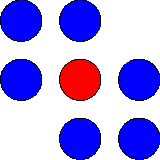
\includegraphics[width=0.17\textwidth , height=0.17\textheight]{pics/2d-7pt/stencil.pdf}}
	\hspace{0.8em}
	\subfloat[Sparsity
	 pattern]{\label{fig:2d-7pt-b}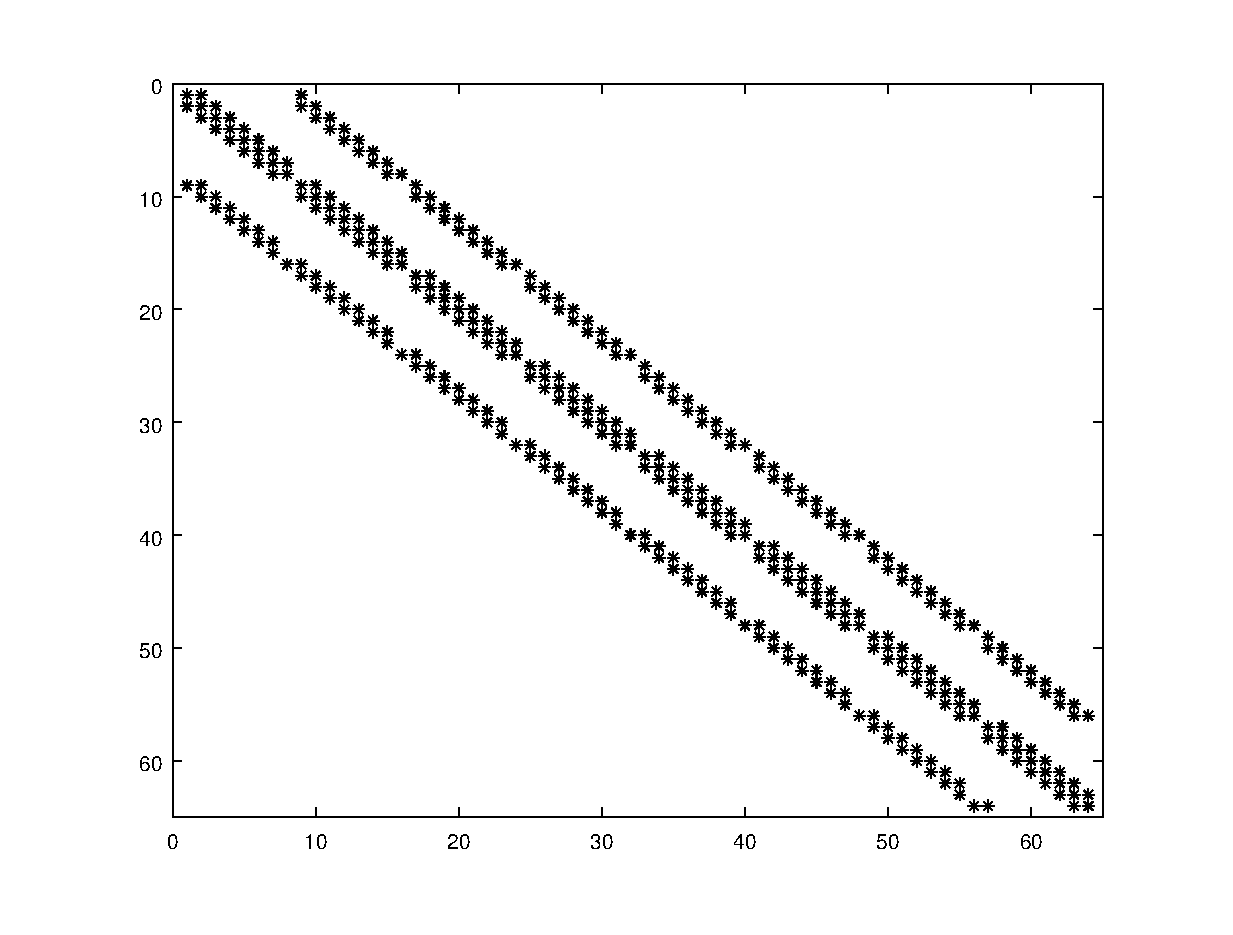
\includegraphics[width=0.38\textwidth , height=0.19\textheight]{pics/2d-7pt/2d_7pt_bw.eps}}
	\hspace{1em}
	\subfloat[Graph]{\label{fig:2d-7pt-c}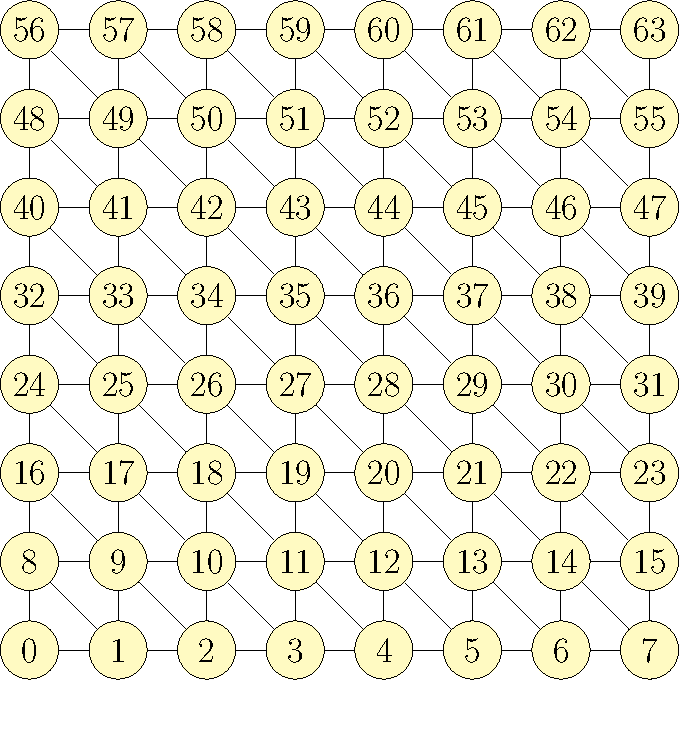
\includegraphics[width=0.32\textwidth , height=0.18\textheight]{pics/2d-7pt/stencil_2d_7pt.pdf}}
	\caption{Basic structure of an artificially designed stencil (a) as well as corresponding sparsity pattern of its matrix discretization (b) and graph representation (c). A $8 \times 8$ lattice in two dimensions with Dirichlet boundary conditions are chosen. The stencil structure is designed for illustration purpose and does not represent any specific application scenario.}
	\label{fig:2d-7pt}
\end{figure}

\subsection*{Definitions}
The following basic definitions from graph theory are used in the following sections:
\begin{itemize}
	\item \textbf{Graph : } $G = (V,E)$ represents a graph where $V(G)$ belongs to set of vertices and $E(G)$ represents the edges in the graph. Note that we use $G$ for irreducible undirected graphs.
	\item \textbf{Neighborhood :} Neighborhood of vertex $u$ represented as $N(u)$ is defined as:
	\begin{equation*}
	  N(u) = \set{ v : uv \in E}.
	\end{equation*}
	\item \textbf{Subgraph :} In this paper a subgraph $H$ of graph $G$ specifically refers to the subgraph induced by vertices $V' \subseteq V(G)$ and is defined as
	\begin{equation*}
		H = (V', \set{ uv : uv \in E(G) \text{ and } u,v \in V'}).
	\end{equation*}
\end{itemize}

\subsection{Level Construction}\label{subsec:LEVEL_CONST}
The first step of \RACE is to determine different \levels in the graph followed by a related permutation of the graph data structure. This is equivalent to well-known bandwidth reduction algorithms such as ``(Reverse) \CMfull" or ``Breadth First Search" (\BFS) \cite{BFS} based approaches. Though the RCM method is implemented in \RACE, we use the  \BFS reordering in the following for better illustration purpose.
%\BFS can also be replaced with better bandwidth reduction algorithms like ``(Reverse) \CMfull".  
As a first step we choose a root vertex which is assigned to the first level ($L(0)$). All other levels ($L(i)$ for $i > 0$) are defined to  contain vertices that are in neighborhood of vertices in previous \level $L(i-1)$ but not in level $L(i-2)$ \cite{BFS_level_def} \ie
\begin{equation}\label{eq:level}
L(i) = 
\begin{cases}
	  u : u \in N(L(i-1)) \cap \overline{N(L(i-2))}  & \text{ if } i \neq 0, \\
	 root & otherwise.
\end{cases}   
\end{equation}

From \cref{eq:level} one finds that the $i$-th \level consist of all vertices that have a minimum distance of $i$ from the root node. See \Cref{alg:BFS} on how to determine minimum distance of each node from the root. The total number of levels obtained with this graph traversal is denoted as \totalLvl. \Cref{fig:2d_7pt_level_construction} shows the {\CA is the reqd.} \totalLvl=14 \levels of an artificial stencil discretization, where the index of each vertex ($v$) refers to the vertex number and the superscript represents the \level number, \ie
\begin{equation}\label{eq:node_notation}
	v^i \implies v \in L(i).
\end{equation}
Note that this is substantially different to the \levels used in ``level-scheduling" \cite{saad} approach which applies a ``Depth First Search".

\begin{figure}[tbhp]
	\centering
	\subfloat[Level construction]{\label{fig:2d_7pt_level_construction}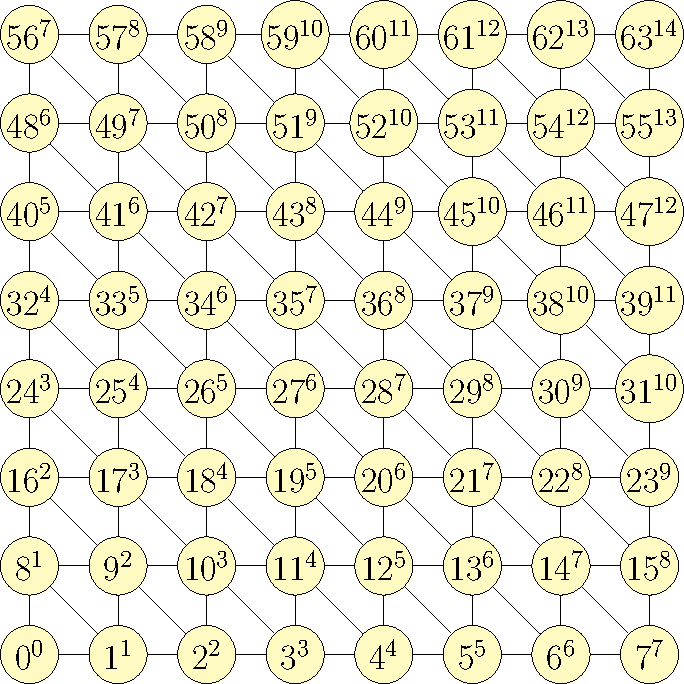
\includegraphics[height=0.18\textheight,width=0.32\textwidth]{pics/level_construction/stencil_2d_7pt}}
	\hspace{1em}
	\subfloat[Permuted graph ($G'$)]{\label{fig:2d_7pt_perm}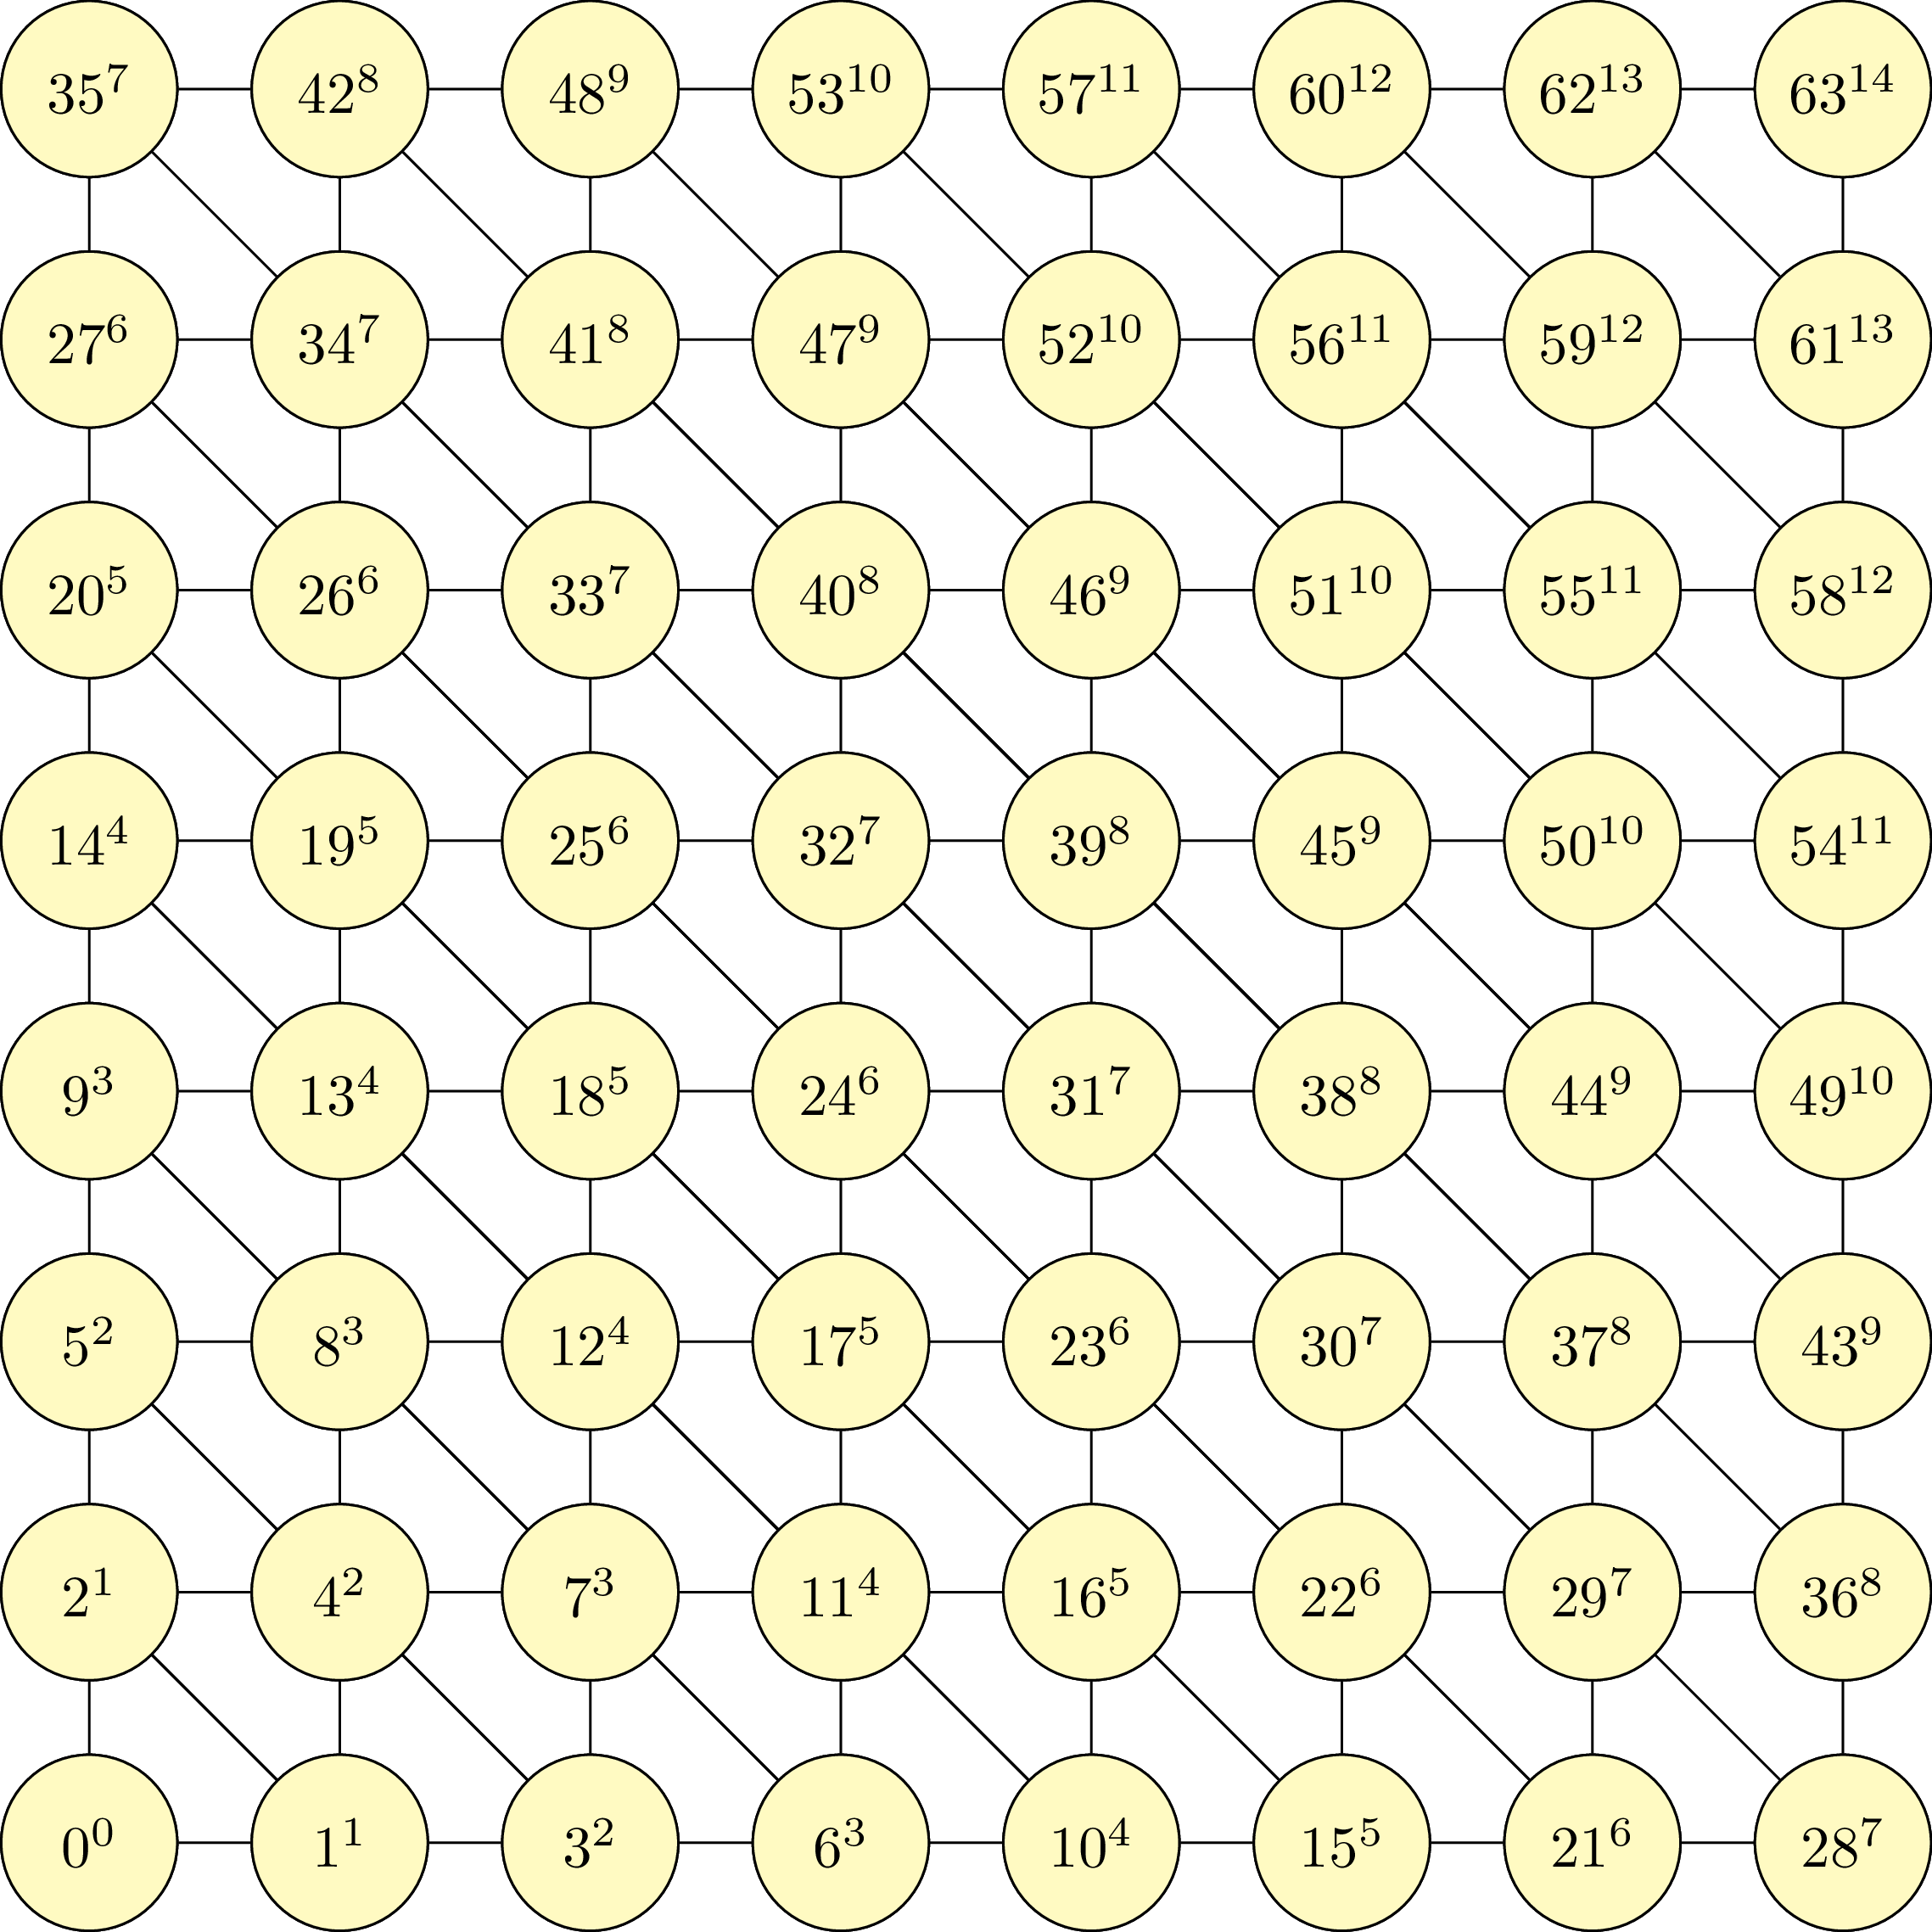
\includegraphics[height=0.18\textheight,width=0.32\textwidth]{pics/permutation/stencil_2d_7pt}}
	\hspace{1em}
	\subfloat[]{\label{fig:2d_7pt_levelPtr}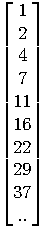
\includegraphics[height=0.18\textheight,width=0.07\textwidth]{pics/permutation/levelPtr}}
	\caption{Levels of the original graph (a) and the permuted graph (b) for the \stex. The entries of  the \levelPtr associated with $G'$ are presented in (c).}
	\label{fig:2d-7pt_step_1_2}
\end{figure}


%\subsection{Permutation}\label{subsec:PERM}
After the \levels have been determined, the matrix is permuted in the order of its \levels, such that the vertices in $L(i)$ are stored consecutively and appear before that of $L(i+1)$. \Cref{fig:2d-7pt_step_1_2} displays the graph ($G' = P(G)$) of \stex after applying this permutation ($P$) and demonstrates the enhanced spatial locality of the vertices within an level (see \cref{fig:2d_7pt_perm}) as compared to the original (lexicographic) numbering (see \cref{fig:2d_7pt_level_construction}).  Until now the procedure is the same as \BFS (or \RCM). 

As \RACE uses information about the \levels for resolving dependencies in the coloring step, we store the entry point to each level in the permuted data structure (of $G'$) in an array $\levelPtr[0:$ \totalLvl$]$, \ie \levels on $G'$ can be identified as:
\begin{equation*}
	L(i) = \set{ u : u \in [\levelPtr[i]:(\levelPtr[i+1]-1)] \text{ and } u \in V(G')} .
\end{equation*}

The entries of \levelPtr for \stex are shown in \cref{fig:2d_7pt_levelPtr}. 
%, and one could easily read from \levelPtr that vertices from $\levelPtr(4)=7$ to $\levelPtr(5)-1=10$ belongs to $L(4)$.
 
 \subsection{Distance-k coloring} \label{subsec:DK}
 The \levels generated above serve as the base for our \DK coloring procedure as they contain information about the neighborhood relation between the vertices of any two levels. Following the definition in~\cite{dist_k_def}, two vertices are called \DK neighbors if the shortest path connecting them consists of at most $k$ edges.
%In this section we introduce the idea of \DK neighbor and show how this idea can be used to color the matrix with the help of the level information that we already have in hand.
This implies $u$ is a \DK neighbor of $v$ (denoted as $u\xrightarrow{k}v$)  if
 \begin{equation}\label{eq:dk}
	  u\xrightarrow{k}v  \iff  v \in \set{ u \cup N(u) \cup N^2(u) \cup ... N^k(u) }.	 
 \end{equation}
 For undirected graphs as considered in this work  $u\xrightarrow{k}v$ also implies $v\xrightarrow{k}u$. Based on this definition we consider two vertices to be \DK independent if they are not \DK neighbors. Thus,  \levels $L(i)$ and $L(i+k+j)$  of the permuted graph $G'$ are \DK independent for all $j\geq1$ as shown in the following:
  \begin{corollary}\label{corollary_dk}
   $L(i)$ and $L(i\pm(k+j))$ are \DK independent $\forall j\geq1$. 
  \end{corollary}
  \begin{proof}
  	We prove by contradiction. Let there exist $u,v \in V(G')$ such that  $u \in L(i)$ and $v \in  L(i \pm (k+j)) \forall j\geq1$. Assume $u,v$ are \DK neighbors ($u\xrightarrow{k}v$). From \cref{eq:level}, \cref{eq:dk} and the fact $G'$ is undirected we get 
  	\begin{align*}
	  	u\xrightarrow{k}v \iff & v \in \set{L(i) \cup L(i \pm 1) \cup ... \cup L(i \pm k)} \\
	  	\implies & v \notin L(i \pm (k+j) \text{  } \forall j \geq 1
  	\end{align*}
  	which contradicts to $v \in L(i \pm (k+j) ) \forall j \geq 1$. This implies $u$ and $v$ are \DK independent.
  \end{proof}

\Cref{corollary_dk} implies that if there is a gap of \emph{\atleast} one \level between any two \levels ($L(i), L(i+2)$ for example) all the vertices between them are \DONE independent. Similarly if the gap consists of \emph{\atleast} two \levels between any two \levels ($L(i), L(i+3)$ for example) we have \DTWO independent levels.
  
 \begin{figure}[tbhp]
 	\centering
 	\subfloat[\DONE independent \levelGroups]{\label{fig:2d_7pt_d1}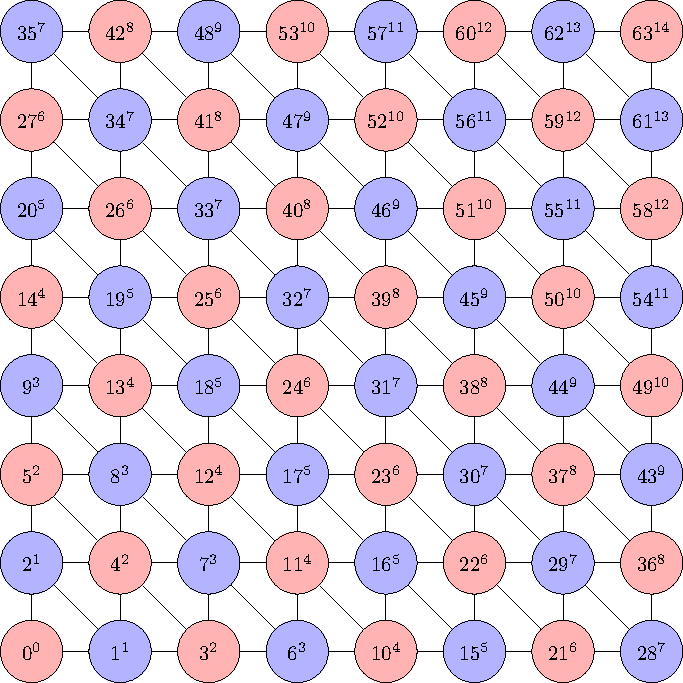
\includegraphics[height=0.2\textheight,width=0.4\textwidth]{pics/dk_coloring/stencil_2d_7pt_d1}}
 	\hspace{2.5em}
 	\subfloat[\DTWO independent \levelGroups]{\label{fig:2d_7pt_d2}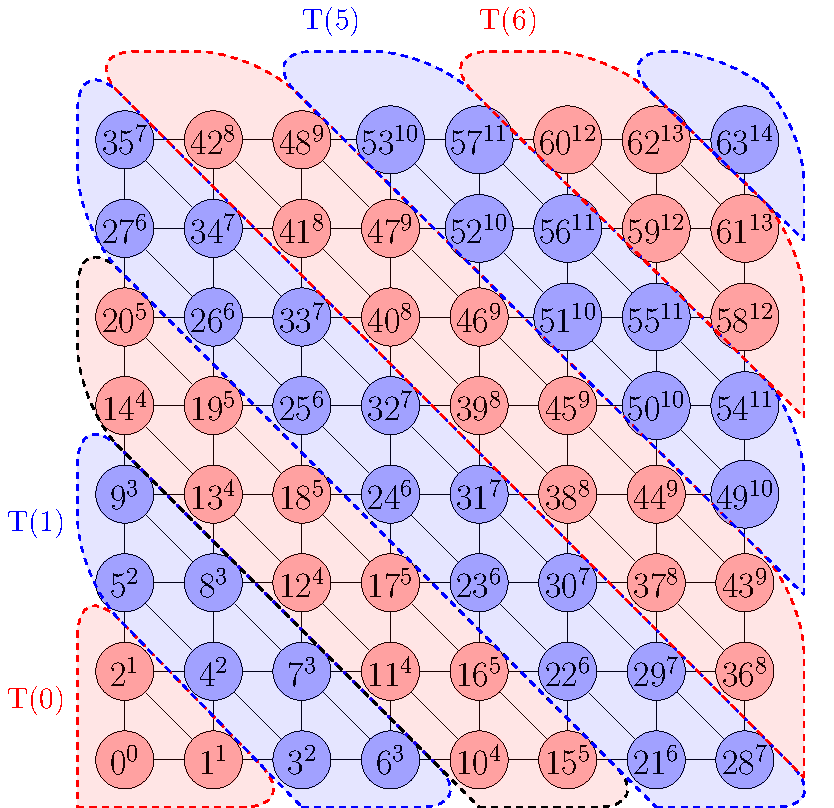
\includegraphics[height=0.23\textheight,width=0.48\textwidth]{pics/dk_coloring/stencil_2d_7pt_d2_with_lg}}
 	\caption{Forming \DONE and \DTWO independent \levelGroups for the \stex.}
 	\label{fig:2d-7pt_d1_d2}
 \end{figure}
 
 % {\CA Maybe more explanation is required.} 
 The weak definition used in \cref{corollary_dk} offers many choices for forming \DK independent sets of vertices, which can then be executed in parallel. 
 In  \Cref{fig:2d_7pt_d1}  and \Cref{fig:2d_7pt_d2} we present one example for \DONE and \DTWO coloring of our \stex, respectively. The \DONE coloring uses a straight forward approach by assigning two colors to alternating levels, i.e. \levels of a color can be calculated concurrently. In case of \DTWO independency we refrain from using three colors but instead aggregate two adjacent \levels to form a \levelGroup (denoted by $T(i)$) and perform a \DONE coloring on top of those groups. This guarantees that vertices of two \levelGroups of the same color are \DTWO independent and can be executed in parallel. Here, the vertices in $T(0)$, $T(2)$, $T(4)$, $T(6)$ can be operated by four different threads in parallel, i.e. one thread per \levelGroup.  After synchronisation the remaining four blue \levelGroups can also be executed in parallel. Note, that within a single \levelGroup all verticies are computed in their original order enabling high spatial locality for accessing them. This idea can be generalized such that for \DK coloring, each \levelGroup contains \atleast $k$ adjacent \levels but the number of levels per \levelGroup may be different. Thus formed \levelGroups are then \DONE colored. Then, all \levelGroups within a color can be executed in parallel. This simple approach allows to generate workload for $\frac{\totalLvlMATH}{2 k}$ threads if \DK coloring is requested.
 
However, choosing the same number of \levels for each \levelGroup may lead to severe load imbalances depending on the matrix structure. In particular the use of bandwidth reduction schemes such as BFS or RCM  will further worsen that problem due to the lens like shape of the reordered matrix leading to low workload for matrix rows at the top and bottom of the matrix. Compare \eg $T(1)$ and $T(7)$ with  $T(3)$ and $T(4)$ in \cref{fig:2d-7pt_d1_d2}.
 %coloring by aggregating consecutive levels into \levelGroups (denoted by $T(i)$). In  \Cref{fig:2d_7pt_d1}  and \Cref{fig:2d_7pt_d2} we present one example for \DONE and \DTWO coloring of our \stex, respectively. The \DONE coloring uses straight forward approach by assigning two colors to alternating levels, i.e. \levelGroup and \level is equivalent here. For and applying a \DONE coloring on top of those groups as shown for \DTWO coloring in \cref{fig:2d_7pt_d2}.  In this context \Cref{fig:2d-7pt_d1_d2} contains two potential colorings for \DONE independent \levels as \DTWO coloring also solves \DONE dependencies.  One could also group some more of nearby \levels together to form a \levelGroup, and make this \DONE or \DTWO independent of other \levelGroups. The $i$-th \levelGroup would be denoted by $T(i)$. Difference between \level and  \levelGroup can be seen in \cref{fig:2d_7pt_d2}, for \cref{fig:2d_7pt_d1} \levelGroup and \level coincides. In principle one could compute on all independent \levelGroups in parallel, but sequentially within a \levelGroup, \ie for example in \cref{fig:2d_7pt_d2} $T(0)$, $T(2)$, $T(4)$, $T(6)$ can be operated by four different threads in parallel and in the next sweep rest \levelGroups. For the configurations seen in \cref{fig:2d-7pt_d1_d2} then we have $\frac{\totalLvlMATH}{2}$ and $\frac{\totalLvlMATH}{4}$ parallelism for \DONE and \DTWO kernels respectively.
  %However the problem with the configurations like the one seen in \cref{fig:2d-7pt_d1_d2} {\CA is that there, check Holger's comment} is load imbalances between threads because the number of rows (\nrows) per \levelGroup is not distributed evenly. As seen here in the case of \stex the threads working on extreme ends of graph (\eg $T(1), T(7)$) have a small amount of work compared to the threads working on middle (\eg $T(3), T(4)$). 
  
  \subsection{Load balancing}\label{subsec:LB}
  Depending on the matrix each \levelGroup contains different number of rows, that leads to load imbalances as seen above in \cref{subsec:DK}. \Inorder to avoid this problem we employ a load balancing scheme. At this step  we plug in details from the hardware side  namely the total parallelism required by the hardware. The idea is to exploit only the required parallelism while at the same time maintain \DK constraint seen in \cref{corollary_dk}. To balance the load more nearby \levels would be added to a \levelGroup ($T(x)$) which has less number of rows ($\nrowsMath(T(x))$) and at \levelGroup where we have considerably big \levels only sufficient amount of \levels to maintain \DK constraint would be assigned. Assigning nearby levels instead of others further helps in preserving data locality. 
  
  An algorithm for load balancing can be found in \cref{alg:LB}. The aim of the algorithm is to reduce combined variance of number of rows ($\nrowsMath(T(i))$) in each \levelGroup $T(i)$. It does this by calculating mean and variance of $T\_size$ in each parallel sweeps, where $T\_size(i)$ is $\nrowsMath(T(i))$(number of rows in $T(i)$). For example in \cref{fig:2d_7pt_d2} we need to calculate mean of $T\_size$ of all \levelGroups in red sweep and blue sweep separately. The combined variance is then found by summing up the variances in each parallel sweep. \Inorder to reduce this combined variance we select the \levelGroup that has biggest absolute deviation from mean and try to add/remove levels to/from this \levelGroup from/to a \levelGroup that has biggest/least signed deviation. While removing \levels from a \levelGroup one has to take care that the \DK coloring is not violated, for example in case of \DTWO and two sweep scheme as seen in \cref{fig:2d_7pt_d2} we need to ensure at least two levels remain in a \levelGroup. To aid this shifting of \levels we use a pointer denoted as $T\_ptr$. $T\_ptr$ points to the beginning of each \levelGroup, therefore shifting them changes the size of \levelGroups. Doing this process in an iterative way finally we end up in a state with lowest combined variance at which no further moves are possible either due to violation of \DK dependency or due to increase in combined variance. \Cref{fig:lb_alg} shows step by step procedure involved in load balancing and \cref{fig:2d_7pt_lb} shows \levelGroups after load balancing applied on \stex of size $16 \times 16.$

  One could also do this entire load balancing based on number of non-zeros (\nnz) rather than \nrows, in this case $T\_size(i)=\nnzMath(T(i))$ (non-zeros in $T(i)$).
  
   \begin{figure}[tbhp]
   	\centering
   	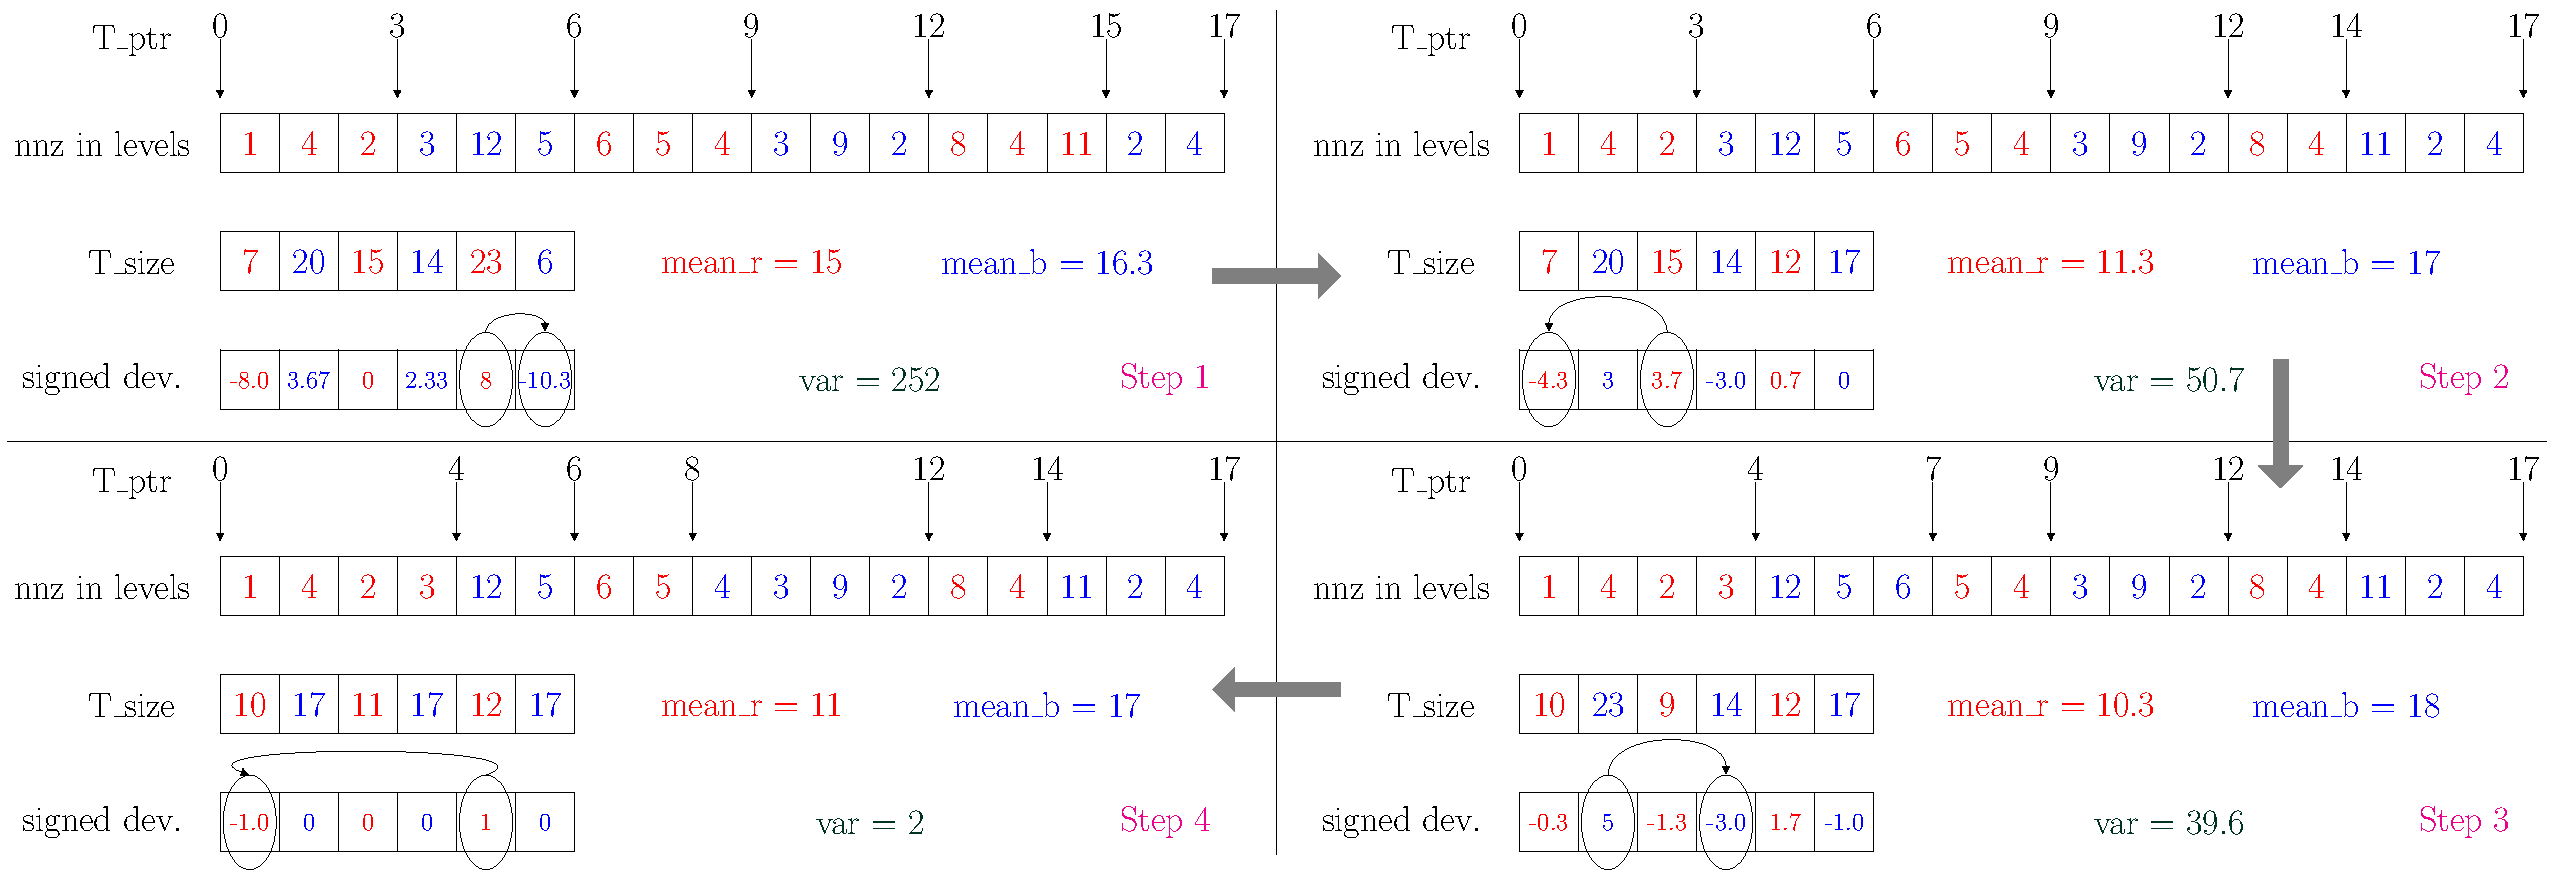
\includegraphics[height=0.22\textheight,width=\textwidth]{pics/load_balancing/lb_alg/lb_all}
   	\caption{Steps in load balancing (clockwise starting from top-left)}
   	\label{fig:lb_alg}
   \end{figure}
   
    
    \begin{figure}
      \begin{minipage}[c]{0.63\textwidth}
      	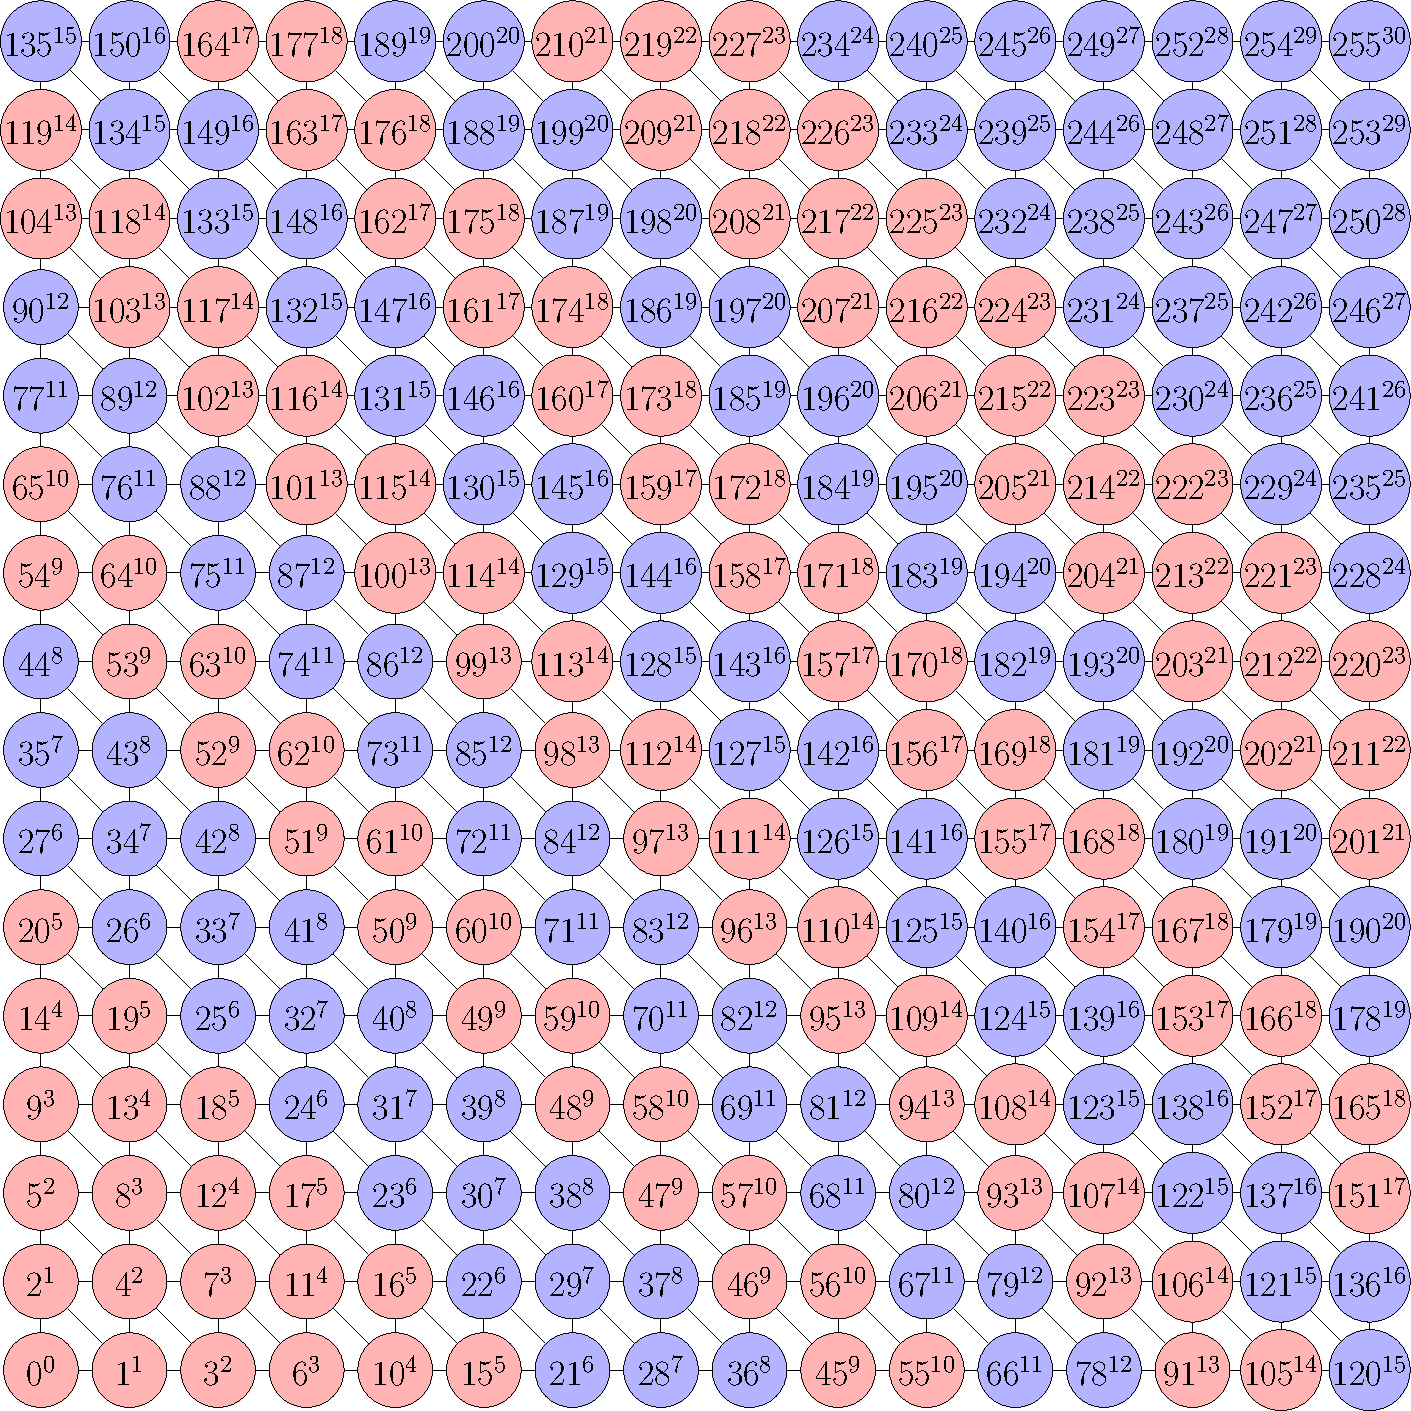
\includegraphics[height=0.26\textheight,width=0.9\textwidth]{pics/load_balancing/2d-7pt/stencil_2d_7pt}
      \end{minipage}\hfill
      \begin{minipage}[c]{0.34\textwidth}
      	\caption{After load balancing for five threads and \DTWO dependency on \stex, domain size $16 \times 16$. Note that \levelGroups at extreme end have more \levels due to less \nrows in each \level, while \levelGroups in middle having bigger \levels maintain two levels to preserve \DTWO constraint.
      	} \label{fig:2d_7pt_lb}
      \end{minipage}
     \end{figure}
     

	\subsection{Recursion}\label{subsec:REC}
	As seen above in \cref{subsec:DK} maximum amount of parallelism by the above approach depends on total number of levels (\totalLvl), also for most of the graphs as we approach the limit of parallelism there is not much room for load balancing, leading to imbalances. Depending on matrix and hardware underneath this might lead to inefficient utilization of resources. \Inorder to avoid this problem we use the concept of recursion and exploit further parallelism if required by the hardware. Idea here is to intelligently select sub-graph(s) of the entire matrix and apply all the three steps recursively on this \subgraph. In the following we will show this concept in the context of \DONE and  later we will extent it to \DK dependencies. In order to explain the basic concepts easily and include all the corner cases we demonstrate the procedure on a simple graph as shown in \cref{fig:rec_d1_s1_a}, later we will show the results of applying recursion on \stex. Further we will discuss on the method employed to select proper sub-graph and to have a globally balanced load.
	
	\subsubsection{Distance-$1$}
	\LevelGroups which we constructed till now belong to first stage of recursion ($s=0$). Stage number of recursion is denoted using subscript, \ie for example $L_s(i)$ denotes \level $i$ of stage $s$. Contrary to methods like \MCfull we didn't require each nodes in a color to be \DONE independent of each other, rather we had a weak constraint as prescribed by \cref{corollary_dk}. Due to this there can exist more parallelism within a \levelGroup. For example in \cref{fig:rec_d1_s1} we see that within third \levelGroup of first stage (T$_0$(2)) vertices $4 \not\xrightarrow{1} 5$ ($4$  \DONE independent to $5$), $4 \not\xrightarrow{1} 6$, $4 \not\xrightarrow{1} 7$ and $5 \not\xrightarrow{1} 7$, implying each of these pairs can be computed in parallel without any \DONE conflicts. This parallelism couldn't be exploited in first stage ($s=0$)  since vertices in $L_0(i)$ (here $i=2$) were connected to preceding \level $L_1(i-1)$ although some of them were not \DONE dependent within $L_0(i)$. \Inorder to exploit this parallelism we use the concept of recursion.
	
     \begin{figure}[thbp]
     	\centering
     	\subfloat[Example graph]{\label{fig:rec_d1_s1_a}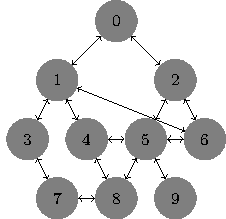
\includegraphics[width=0.26\textwidth, height=0.14\textheight]{pics/recursion/d1/rec_graph_s1/recursion_graph_1}}
     	\hspace{1.5em}
     	\subfloat[Stage 1 levels in graph]{\label{fig:rec_d1_s1_b}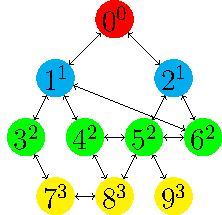
\includegraphics[width=0.26\textwidth, height=0.14\textheight]{pics/recursion/d1/rec_graph_s1/recursion_graph_2}}
     	\hspace{1.5em}
     	\subfloat[\DONE coloring]{\label{fig:rec_d1_s1_c}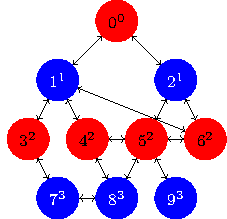
\includegraphics[width=0.26\textwidth, height=0.14\textheight]{pics/recursion/d1/rec_graph_s1/recursion_graph_3}}
        \caption{Shows potential for more parallelism. $T_0(1),T_0(2)$ and $T_0(3)$ has more parallelism. Note that the graph shown here is not related to the previous \stex.}
     	\label{fig:rec_d1_s1}
     \end{figure}
     
     Recursion begins by selection of a \subgraph of the matrix. A typical choice is a \subgraph induced by vertices in a \levelGroup of previous stage, more on the selection of \subgraph will be seen later in \cref{subsec:subgraph_selection}. For example let's choose \subgraph induced by $T_0(2)$ for recursion. The chosen \subgraph can be isolated from rest of the graph since  \DONE coloring step in stage 0 has already made \levelGroups in a sweep independent of each other. Now we just need to repeat all the three steps explained previously (\cref{subsec:LEVEL_CONST} - \cref{subsec:LB}) to exploit parallelism within this \subgraph.
   
     \begin{figure}[thbp]
     	\centering
     	\subfloat[]{\label{fig:rec_d1_s2_a}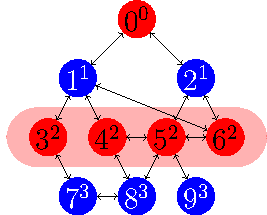
\includegraphics[width=0.26\textwidth, height=0.14\textheight]{pics/recursion/d1/rec_graph_s2/recursion_graph_stage2_1}}
     	\hspace{2.25em}
     	\subfloat[]{\label{fig:rec_d1_s2_b}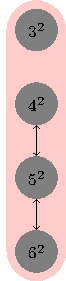
\includegraphics[width=0.08\textwidth, height=0.14\textheight]{pics/recursion/d1/rec_graph_s2/recursion_graph_stage2_2}}
     	\hspace{1.75em}
     	\subfloat[]{\label{fig:rec_d1_s2_c}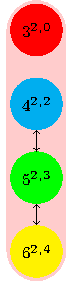
\includegraphics[width=0.07\textwidth, height=0.14\textheight]{pics/recursion/d1/rec_graph_s2/recursion_graph_stage2_3}}
     	\hspace{1.75em}
     	\subfloat[]{\label{fig:rec_d1_s2_d}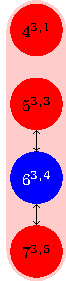
\includegraphics[width=0.07\textwidth, height=0.14\textheight]{pics/recursion/d1/rec_graph_s2/recursion_graph_stage2_4}}
	     \hspace{1.75em}
	     \subfloat[]{\label{fig:rec_d1_s2_e}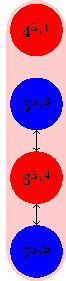
\includegraphics[width=0.07\textwidth, height=0.14\textheight]{pics/recursion/d1/rec_graph_s2/recursion_graph_stage2_5}}
     	\caption{Shows recursion being applied to $T_0(2)$. \Cref{fig:rec_d1_s2_b} shows the selected \subgraph, \cref{fig:rec_d1_s2_c} shows level construction step on the \subgraph, \cref{fig:rec_d1_s2_d,fig:rec_d1_s2_e} shows two possibility of \DONE coloring of the \subgraph}
     	
     	\label{fig:rec_d1_s2}
     \end{figure}
     
     \Cref{fig:rec_d1_s2} shows an illustration of applying second stage ($s=1$) of recursion on $T_0(2)$. To incorporate the information of levels in different stages of recursion onto the vertices we extent the definition in \cref{eq:node_notation} to the following:
	 \begin{equation}
	    v^{i,j,k...} \implies v \in \set{L_1(i) \cap L_2(j) \cap L_3(k) \cap ...} 
	 \end{equation}
	 
     In this case at the end of recursion (\cf \cref{fig:rec_d1_s2_d}, \cref{fig:rec_d1_s2_e}) on $T_0(2)$ we obtain parallelism for two more threads. Note that the \subgraphs might have multiple islands (group of vertices in a graph that are not connected to rest of the graph). For example vertex 3 in \cref{fig:rec_d1_s2_b} is an island in the considered \subgraph, similarly vertices 4,5,6 combine to form an island. Since an island is totally disconnected from the rest of the graph it can be executed in parallel to rest of the graph. To take advantage of this the starting node in next island is assigned with an increment of two levels, as seen in \cref{fig:rec_d1_s2_c}. Due to this there exists multiple valid \DONE configuration (\cf \cref{fig:rec_d1_s2_d,fig:rec_d1_s2_e}) and the selection of the optimal one will be done in the final load balancing step of a particular stage as described in \cref{subsec:LB}.    
     
     With this recursive process we were able to find independent \levelGroups ($T_{s+1}$) within \levelGroup of previous stage ($T_s$) and therefore the thread which works on $T_s$ has to spawn threads to parallelize within $T_{s+1}$.
     
	\subsubsection{Distance-$k$}
	For \DK the same procedure as \DONE applies, except with a slight difference in selecting the \subgraph. In \DONE we considered \subgraphs induced by \levelGroups, but for \DK coloring this is not sufficient. As seen in \cref{fig:rec_d2_wrong} for \DTWO coloring the selection of $T_0(1)$ as \subgraph did not guarantee \DTWO independency within \levelGroup $T_1$ of the \subgraph, for \eg $T_1(0)$ and $T_1(2)$ are not \DTWO independent (\cf \cref{fig:rec_d2_wrong_d}). This is due to the fact that for $k>1$ dependencies two vertices $a,b$ within a \subgraph might be connected to a common vertex ($c$) outside the \subgraph leading to a \DK dependency between $a$ and $b$. In \cref{fig:rec_d2_wrong} we see 	$3 \xrightarrow{1} 1 \text{ \& } 6 \xrightarrow{1} 1 	\implies 3 \xrightarrow{2} 6$, but since vertex $2$ was not in the \subgraph considered we missed this dependency. 

	
     \begin{figure}[thbp]
     	\centering
     	\subfloat[]{\label{fig:rec_d2_wrong_a}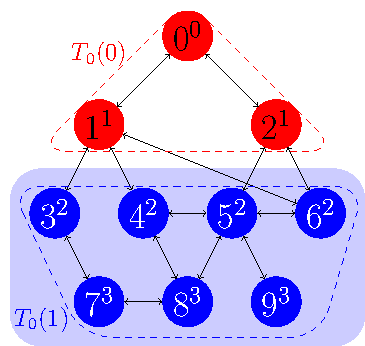
\includegraphics[width=0.23\textwidth, height=0.13\textheight]{pics/recursion/d2/wrong/recursion_graph_wrong_1}}
     	\hspace{0.6em}
     	\subfloat[]{\label{fig:rec_d2_wrong_b}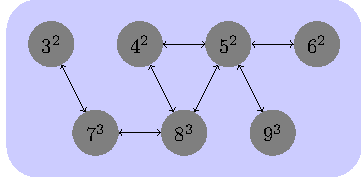
\includegraphics[width=0.23\textwidth, height=0.07\textheight]{pics/recursion/d2/wrong/recursion_graph_wrong_2}}
     	\hspace{0.6em}
     	\subfloat[]{\label{fig:rec_d2_wrong_c}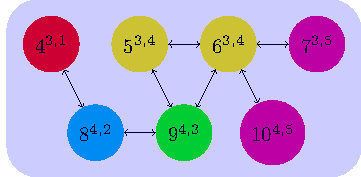
\includegraphics[width=0.23\textwidth, height=0.07\textheight]{pics/recursion/d2/wrong/recursion_graph_wrong_3}}
     	\hspace{0.6em}
     	\subfloat[]{\label{fig:rec_d2_wrong_d}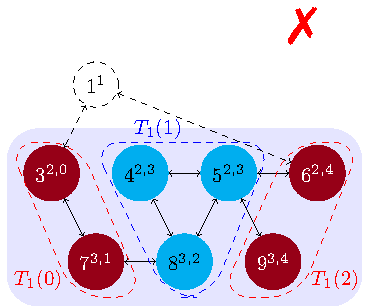
\includegraphics[width=0.23\textwidth, height=0.13\textheight]{pics/recursion/d2/wrong/recursion_graph_wrong_4}}
     	\caption{\Cref{fig:rec_d2_wrong_a,fig:rec_d2_wrong_b} shows \levelGroup induced \subgraph selected for recursion in case of \DTWO. But applying the three steps to this selected \subgraph does not guarantee a \DTWO independency between \levelGroup of same sweep (color) as seen in \cref{fig:rec_d2_wrong_d}}
     	\label{fig:rec_d2_wrong}
     \end{figure}
   
   \Inorder to resolve such dependency we have to consider an extra $(k-1)^{th}$ interface level(s) of the selected \subgraph for the level construction step. The $k^{th}$ interface level(s) of subgraph $T_s(j)$, denoted as $I^k(T_s(j))$, is defined as follows:
   \begin{equation*}
	   I^k(T_s(j)) = \set{u : u \xrightarrow{k} v \text{  } \forall v \in T_s(j) \text { and } u \notin T_s(j)}
   \end{equation*}
   For \DTWO this would mean we have to include $1^{st}$ interface level, the new selection is illustrated in \cref{fig:rec_d2_correct}. If we then do all the three steps with the newly created \subgraph, the final result will preserve \DTWO coloring (see \cref{fig:rec_d2_correct_c}). In the example it can be observed vertices $3$ and $6$ which previously had same color now get assigned to different colors (see \cref{fig:rec_d2_correct_d}). Note that the interface levels have to be considered only in the first step namely level construction in the rest of the steps we just need to consider target \subgraphs induced by \levelGroups \ie in \cref{fig:rec_d2_correct} the \subgraph induced by $T_0(1)$. 
   
     
     \begin{figure}[thbp]
     	\centering
     	\subfloat[]{\label{fig:rec_d2_correct_a}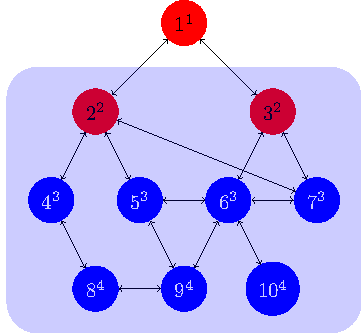
\includegraphics[width=0.22\textwidth, height=0.13\textheight]{pics/recursion/d2/correct/recursion_graph_correct_1}}
     	\hspace{0.6em}
     	\subfloat[]{\label{fig:rec_d2_correct_b}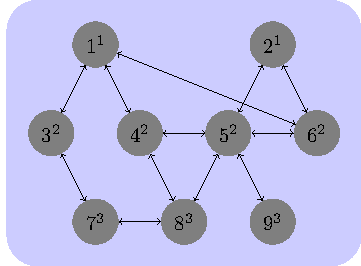
\includegraphics[width=0.22\textwidth, height=0.105\textheight]{pics/recursion/d2/correct/recursion_graph_correct_2}}
     	\hspace{0.6em}
     	\subfloat[]{\label{fig:rec_d2_correct_c}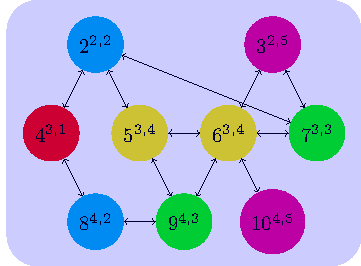
\includegraphics[width=0.22\textwidth, height=0.105\textheight]{pics/recursion/d2/correct/recursion_graph_correct_3}}
     	\hspace{0.6em}
     	\subfloat[]{\label{fig:rec_d2_correct_d}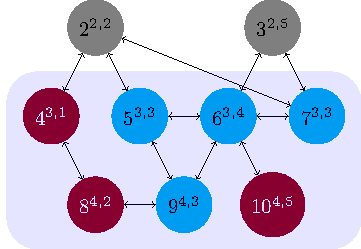
\includegraphics[width=0.22\textwidth, height=0.105\textheight]{pics/recursion/d2/correct/recursion_graph_correct_4}}
     	\hspace{0.6em}
     	\caption{Correct procedure of selecting \subgraph for \DTWO coloring. The \levelGroup $T_0(1)$ and it's $1^{st}$ interface level is chosen as the \subgraph as shown in \cref{fig:rec_d2_correct_a,fig:rec_d2_correct_b}. Level construction step is then applied to this \subgraph as seen in \cref{fig:rec_d2_correct_c}. Rest of the steps like permutation and \DK coloring is applied only to the \subgraph  chosen for recursion (here $T_0(1)$). Finally as seen in \cref{fig:rec_d2_correct_d} we get three \levelGroups at the end of recursion on $T_0(1)$.}
     	\label{fig:rec_d2_correct}
     \end{figure}
     

       \begin{figure}[H]
       	\begin{minipage}[c]{0.6\textwidth}
       		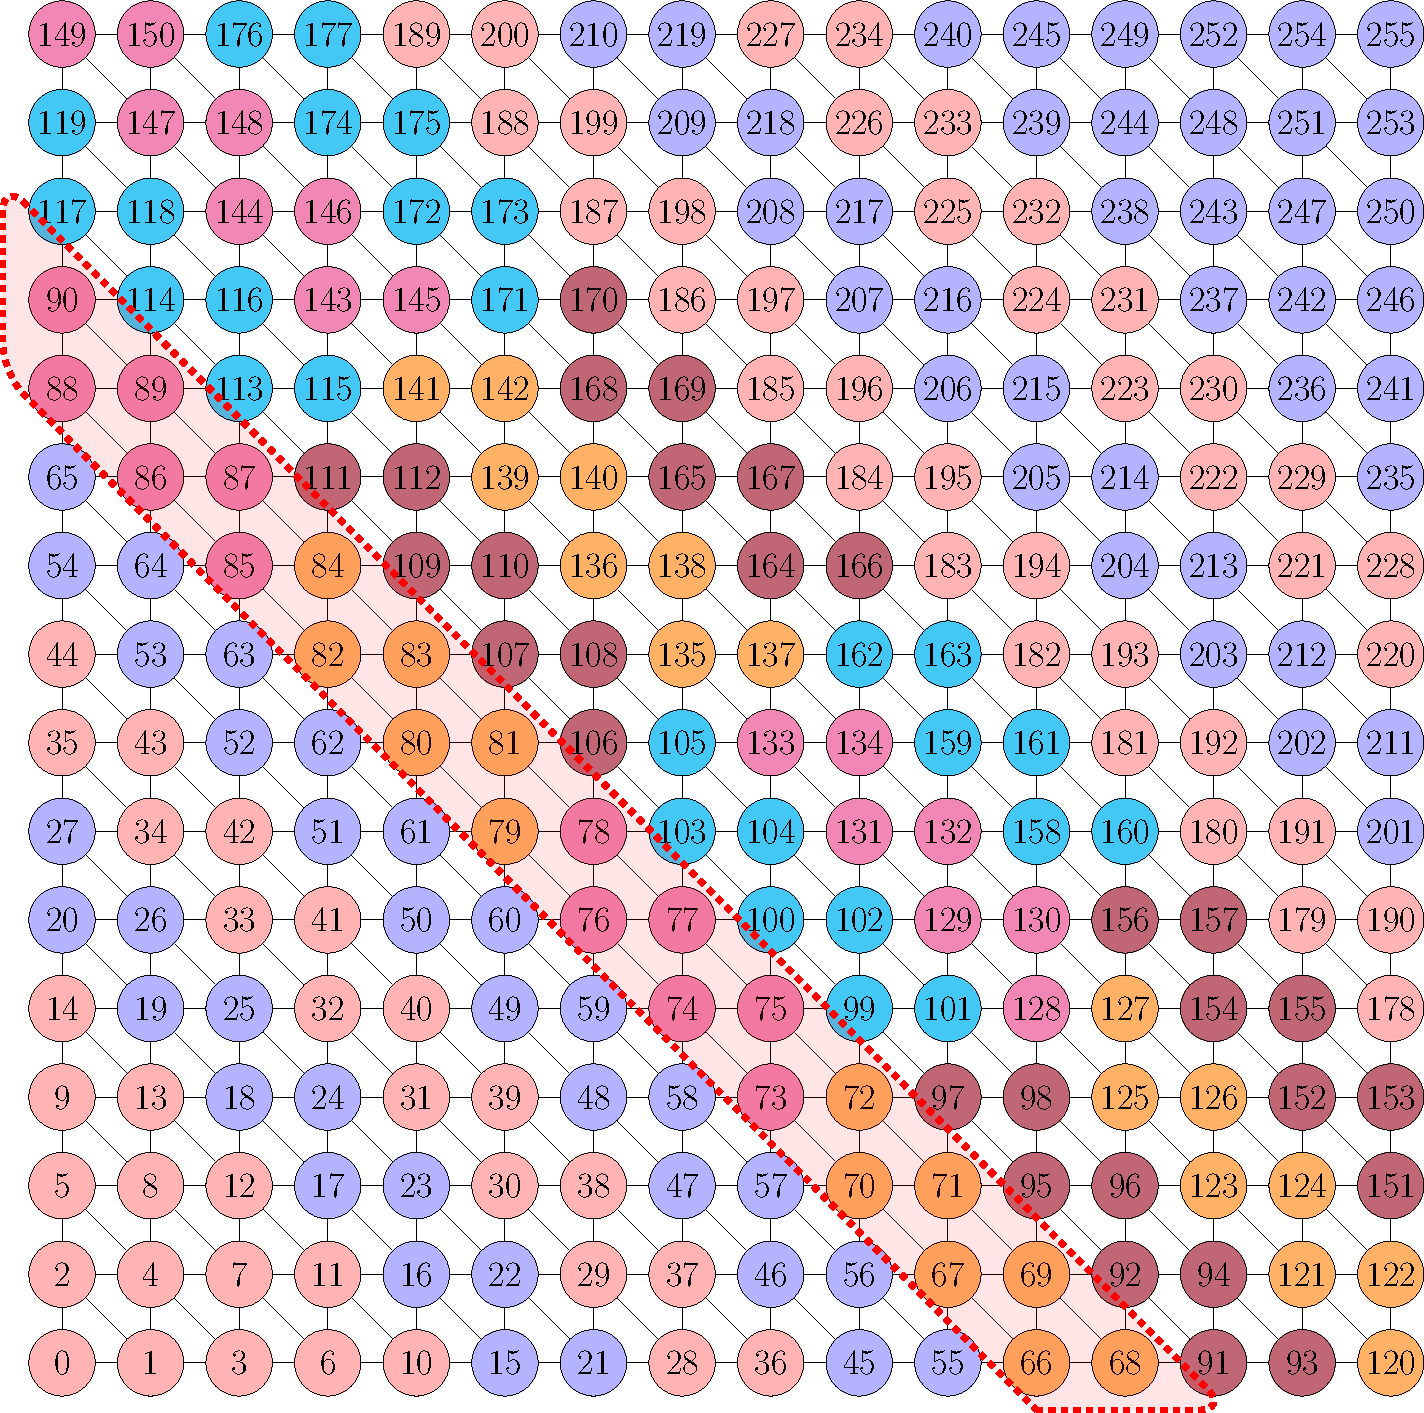
\includegraphics[height=0.3\textheight,width=0.89\textwidth]{pics/recursion/2d-7pt_example/2d-7pt/stencil_2d_7pt}
       	\end{minipage}\hfill
       	\begin{minipage}[c]{0.4\textwidth}
       	%	{\tt for parallel all \textcolor{red}{red}\\
       	%		\hspace*{1em} for parallel all \textcolor{amber}{orange}\\
       	%		\hspace*{1em} for parallel all \textcolor{magenta}{pink}\\
       	%	}
       	%	{\tt for parallel all \textcolor{blue}{blue}\\
       	%		\hspace*{1em} for parallel all \textcolor{carmine}{brown}\\
       	%		\hspace*{1em} for parallel all \textcolor{cyan}{cyan}\\
       	%	}
	       	\begin{tabular}{l|l}
	    %   		\toprule
	       		{No recursion} & {$s=1$ recursion}\\
	       		\midrule
	       	   \multirow{2}{*}{\textcolor{red}{red}} & {\textcolor{amber}{orange}}\\
	       	   \cmidrule(lr){2-2}
	       		& {\textcolor{magenta}{pink}}\\
	       		\midrule
	       	   \multirow{2}{*}{\textcolor{blue}{blue}} & {\textcolor{carmine}{brown}}\\
	       	   \cmidrule(lr){2-2}
	       	   & {\textcolor{cyan}{cyan}}\\
	       	   \bottomrule
	       	\end{tabular}
       		\caption{Recursion applied to \stex for eight threads. Here recursion is applied on \levelGroups $T_1(4-7)$, to get two threads each. The execution order of different \levelGroup is specified in the illustration towards right. Vertical line distinguishes between \levelGroups with and without recursion and each horizontal line denotes the required synchronization. Note the requirement of nested parallelism.}
       		\label{fig:rec_2d-7pt_graph}
       	\end{minipage}
       \end{figure}
     
     \Cref{fig:rec_2d-7pt_graph} (left) shows \DTWO coloring of \stex  for eight threads. Here we see recursion is applied to \levelGroups $T_0(4),T_0(5),T_0(6)$ and $T_0(7)$. In this case each of the \levelGroups where recursion is applied spawns parallelism for two threads. The selection of \levelGroups to refine and number of threads needed from each recursion are determined using a global load balancing technique as will be explained in \cref{subsec:subgraph_selection}.
     
      \Cref{fig:rec_2d-7pt_graph} (right) shows the execution order of different \levelGroups. Note the usage of nested parallelism, \ie for example thread responsible for $T_0(4)$ spawns two child threads to execute $T_1(0) \subset T_0(4)$ and $T_1(2) \subset T_0(4)$ in one parallel sweep, and $T_1(1) \subset T_0(4)$ and $T_1(3) \subset T_0(4)$ in next parallel sweep. At the end of each sweep there is synchronization between threads assigned to \levelGroup of similar color. Since each of the leaf need to synchronize only with it's siblings (leaves of same parent)  we use simple point to point synchronization scheme. 
          
       
	\subsubsection{Internal representation of recursively generated \boldmath{\levelGroups}} \label{subsec:level_tree}
	The recursive nature of our procedure allows to exploit more parallelism. However this introduces more complexity and one has to additionally respect the dependencies between stages and still observe the dependencies within one stage. The best idea is to have a data structure similar to the recursion, therefore we extent the \levelPtr data structure to a hierarchical tree data structure to store these informations. This data structure is called a \levelTree. The root of \levelTree contains information of entire domain, first child leaves of this root \ie leaves with depth 1 stores information about \levelGroups in first stage ($T_0(..)$), leaves with depth 2 stores information about \levelGroups in second stage ($T_1$) and so on. 
	
	 \begin{figure}[thbp]
		 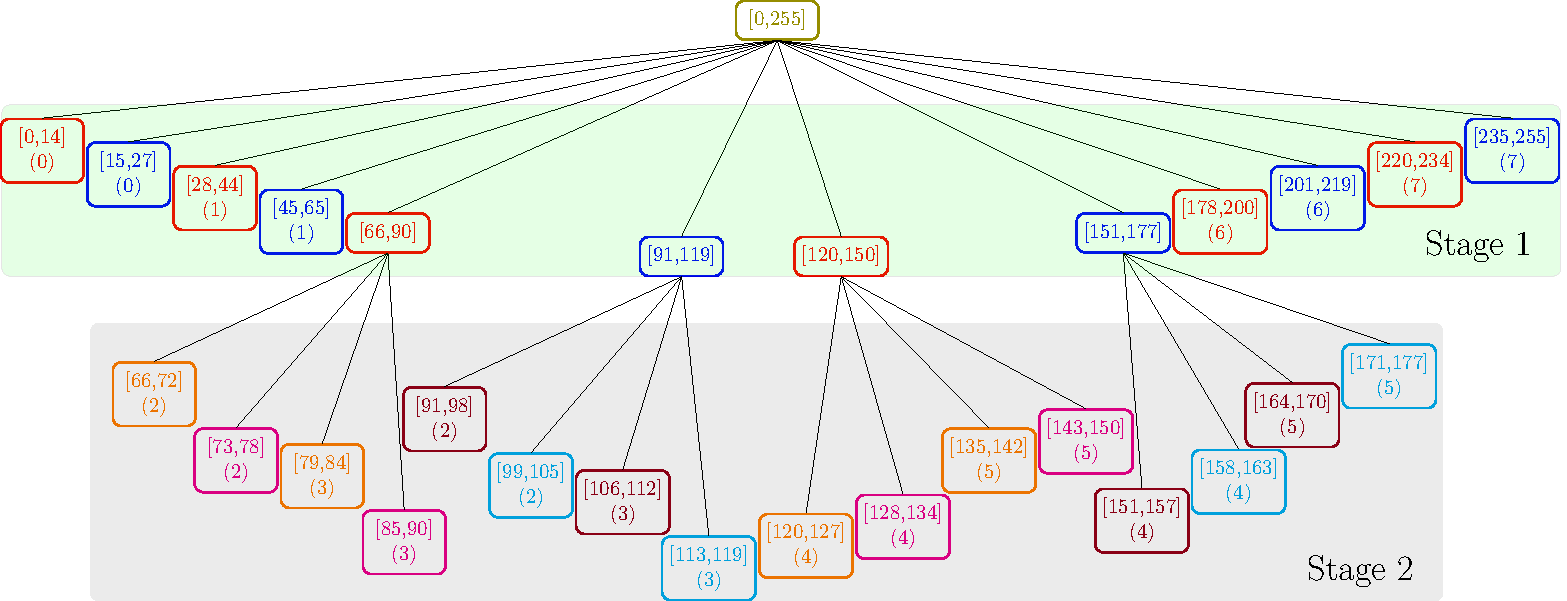
\includegraphics[width=\textwidth, height=0.2\textheight]{pics/recursion/2d-7pt_example/tree/tree}
	 	\caption{\levelTree corresponding to \stex for domain size $16 \times 16$, and 8 threads. The range (square brackets) specified in each leaves represent the vertices belonging to each \levelGroup, the \nrowsEff (see \cref{Sec:param_study}) is represented within angle brackets, and the id refers to the thread id assigned to each \levelGroups assuming compact pinning .}
	 	\label{fig:rec_2d-7pt_tree}
	 \end{figure}

 
 \Cref{fig:rec_2d-7pt_tree} shows a \levelTree corresponding for \stex  with 8 threads as seen in \cref{fig:rec_2d-7pt_graph}. The leaves in the tree correspond to different \levelGroups and store various informations like the range of vertices or nodes that belong to this \levelGroup, the effective number of rows (\nrowsEff) that describes the quality of the method (which we will see later in \cref{Sec:param_study}), and other informations like threads assigned to specific \levelGroups.  Threads are assigned to each \levelGroup depending on the pinning strategy used. For example in \emph{fill} type pinning strategy one would pin thread 0 to $T_0(0)$ and $T_0(1)$, thread 1 to $T_0(2)$ and $T_0(3)$, thread 2 to $T_1(0)  \subset T_0(4)$, $T_1(1) \subset T_0(4)$, $T_1(0)  \subset T_0(5)$ and $T_1(1) \subset T_0(5)$, and so on as seen in \cref{fig:rec_2d-7pt_tree}. 
 
 Note that the \levelTree has a data structure that represents the nested parallelism being used as seen in \cref{fig:rec_2d-7pt_graph} (right). Therefore threads are spawned based on this \levelTree allowing for easy implementation of point to point synchronizations.

\subsubsection{Sub-graph selection and global load balancing} \label{subsec:subgraph_selection}
Parallelism required for hardware underneath can be obtained either by expanding the \levelTree horizontally \ie increasing \levelGroups within a stage or by expanding \levelTree vertically with the help of recursion. But as we have seen before in \cref{subsec:DK} the horizontal parallelism is limited and after a certain extent this would lead to load balancing. Similarly excessive usage of recursion is also not a good idea since data locality worsens due to local permutations within \subgraph. Therefore it is vital to find a proper balance and choose proper configuration. Furthermore just doing load balancing within a single stage is not the best, for example if we had equally balanced within stage 1 in \cref{fig:rec_2d-7pt_tree}, we would receive no benefit from recursion. Therefore a global load balancing becomes inevitable.

\Inorder to select proper \subgraph and do global load balancing we employ a simple algorithm to find proper weights for each \levelGroup ($T_s(i)$) in a particular stage, then depending on this weights, denoted as $w(T_s(i))$, we do load balancing with weights in the particular stage (as seen in \cref{alg:LB}, except weightage is given to \levelGroups). Finally if $w(T_s(i)) > 1$ we use recursion to achieve $w(T_s(i))$ parallel work in the next stage of $T_s(i)$. The basic structure of the algorithm employed to find weights for the first stage is as follows:
\begin{enumerate}
	\item Find weights, $w(L_0(i))$ for each level in the current stage ($s$) by
		\begin{align*}
			w(L_0(i)) &= (\levelPtr_0[i+1] - \levelPtr_0[i])*\frac{\nthreadsMath}{\nrowsMath^{total}}\\
			\nthreadsMath &: \text{total parallelism required by hardware}\\
			\nrowsMath^{total} &: \text{number of vertices in graph}
		\end{align*}
	
	\item Starting from $w(L_0(0))$ sum up weights till they form a number ($a$) close to whole number ($b$). The closeness can be controlled by an efficiency parameter for stage $s$, $\epsilon_s$ is defined as:
	\begin{equation} \label{eq:epsilon}
		\epsilon_s =  1 - abs(a-b);
	\end{equation}
	All the \levels that are involved in the sum belongs to \levelGroups  operated by first thread in the current stage. The obtained number $b$ is chosen as weight for these \levelGroups \ie $w(T_0(0))=w(T_0(1))=b$. A local search is then done by increasing \levels in this \levelGroups to see if there is a better choice ($a$ close to $b$) with weight $b$, finally \levelGroups are formed with the best choice.  The weight for next \levelGroups are found by resetting the sum counter to zero and repeating the  procedure with \levels just after the current \levelGroups.
\end{enumerate}
For other recursive stage ($s\geq1$) same procedure can be applied to find weights $w(T_s(i))$, except that now $\nthreadsMath$ and $\nrowsMath^{total}$ has to be substituted with the threads required and vertices in the \subgraph considered.